\chapter{Evaluation and Results}
\label{chap:evaluation}
\section{Introduction}
\section{Evaluation Metrics}
\section{Iterative Results Summary}
\section{Final Per-Model Results}
\section{Ablation Study}
\section{Synthetic Data Impact}
\section{RL Agent Final Results}
\section{Comparison with State-of-the-Art}
\section{Simulation Results}
\label{sec:sim-results}

The simulation results presented here come from the same Caldera-driven
lab introduced in chapter~\ref{chap:implementation}, replayed against
the production CAVIX stack. They are the only end-to-end measurements
in this thesis: the model-level metrics of the earlier sections
evaluate each component in isolation, while the run described below
exercises the full pipeline, from raw kernel syscall through
detection, reinforcement-learning decision, deterministic gating,
persistence, and analyst-facing fan-out, as a single moving system.

\subsection{Environment}
\label{sec:sim:env}

CAVIX was evaluated end-to-end on a self-contained adversary-emulation
laboratory whose entire stack ran locally on a single Kali Linux
2026.1 host (kernel 6.16, \texttt{x86\_64}). Running the full stack
on one machine rather than against a cloud back-end removed
provider-side variability from the measurements, gave the runner
deterministic control over network conditions, and kept every
artefact (container image, model weight, configuration) reproducible
from the same Docker \cite{docker2024} Compose files committed to
the repository.

The laboratory was split across two isolated bridge networks, as
summarised in figure~\ref{fig:ch5:lab-env}.
\texttt{strix\_lab\_net} hosted the four-container attack range and
the sensing stack: a MITRE ATT\&CK \cite{mitre_attack} adversary
driven by a Caldera C2 server \cite{caldera2024}, two Ubuntu victims
(\texttt{strix\_victim1} and \texttt{strix\_victim2}) running the
Sandcat agent alongside the Linux Auditd subsystem
\cite{auditd2024} and a Wazuh agent (version~4.9.2)
\cite{wazuh2024}, a separate \texttt{strix\_attacker} container
driving external Reconnaissance traffic (T1595, active scanning)
through scripted SSH probe bursts, and the centralised Wazuh
Manager whose decoders normalised the resulting events into
\texttt{/var/ossec/logs/alerts/alerts.json}, tailed by a
co-located Filebeat sidecar \cite{filebeat2024}. The second
network, \texttt{strix\_platform\_net}, hosted the CAVIX detection
stack: a TimescaleDB instance \cite{timescaledb2024} for the
time-partitioned detection records, a Redis~7 instance
\cite{redis2024} for the streaming bus and ephemeral state, the
eight-process CAVIX application stack launched through the Honcho
process manager (FastAPI \cite{fastapi2024}, the Redis-list
bridge worker, the feature normaliser, the inference worker hosting
the five neural models, the verdicts writer materialising
detections in PostgreSQL \cite{postgres2024}, an ARQ background-job
runner, an isolation responder, and an intel-feeds worker), and the
Next.js \cite{nextjs2024} web frontend on port~5600.

\begin{figure}[H]
  \centering
  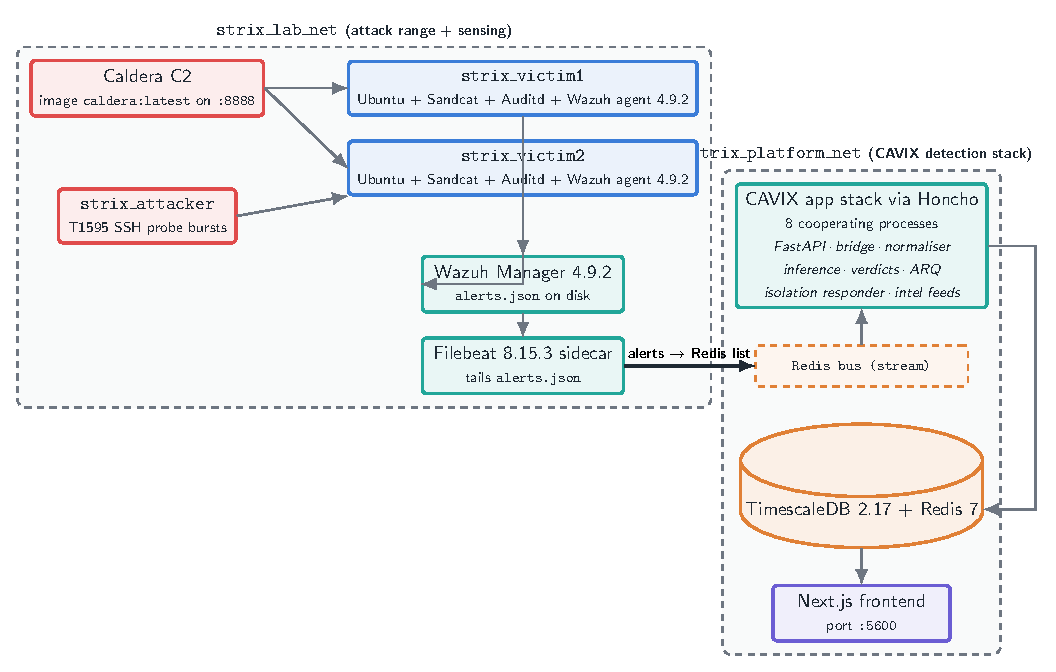
\includegraphics[width=0.95\textwidth]{figures/ch5/tikz/lab_environment}
  \caption{Two-network layout of the evaluation laboratory.}
  \label{fig:ch5:lab-env}
  \par\medskip
  In figure~\ref{fig:ch5:lab-env}, the dashed \texttt{strix\_lab\_net}
  zone on the left hosts the four-container attack range and the
  sensing stack, while the dashed \texttt{strix\_platform\_net} on
  the right hosts the CAVIX detection stack; the only data path
  between the two networks is the alerts-to-Redis hop from the
  Filebeat sidecar to the platform bus.
\end{figure}

Telemetry passed through the pipeline in a single direction. A
syscall on a victim was captured by Auditd, decoded by the local
Wazuh agent, forwarded to the Wazuh Manager, and emitted as a JSON
alert. A sidecar Filebeat (version~8.15.3) \cite{filebeat2024}
tailed the alert file and pushed each line into a Redis list, which
the bridge worker drained onto a Redis stream. The normaliser, the
inference worker, and the verdicts writer consumed that stream in
sequence. Every event terminated as four correlated rows in the
database: the raw alert, the detection carrying all five model
outputs, an attack-chain membership entry, and, when the chain
decider authorised the full pipeline, a Deep Q-Network action
record. End-to-end latency from syscall to dashboard stayed below
five seconds under the nominal load of the runs reported here.

The simulation was launched through \texttt{jury\_demo.sh} with the
\texttt{--non-monotonic} flag, which selected a hand-tuned kill-chain
schedule rather than a strictly forward walk through the MITRE Cyber
Kill Chain. The schedule ran through nine stage transitions in the
order \texttt{[1, 3, 4, 5, 1, 3, 4, 5, 7]}, namely Reconnaissance,
Delivery, Exploitation, Installation, a backward transition to a
second Reconnaissance burst, followed by Delivery, Exploitation,
Installation, and Impact (T1485~/~T1486). The non-monotonic choice
was made for three reasons. First, it matched the empirical
distribution of attack sequences on which the Transformer and the
DQN had been trained, both of which had observed forward and
backward state transitions during training. Second, traversing
Installation (CKC~=~5) twice produced two opportunities for the
safety gate to authorise an \texttt{ESCALATE} on the same chain,
exercising the gate ladder under realistic conditions rather than a
single threshold crossing. Third, terminating at Impact (CKC~=~7)
carried a single coherent attack narrative across the full
kill-chain length. Each Caldera operation used the default atomic
planner; the link-execution timeout was configured so that every
ability either completed or failed cleanly within a per-tactic
budget of roughly forty seconds.

\subsection{Attack Scenarios}
\label{sec:sim:scenarios}

Figure~\ref{fig:ch5:sim:attack-during} captures the dashboard during
the active attack window, before any reinforcement-learning
intervention has been issued. The two parallel timelines correspond
to the two victims and show the same kill-chain stage sequence in
progress, from Reconnaissance through Defense Evasion, Privilege
Escalation, and Persistence. The header counters report a
system-integrity index of 80\,\%, a throughput of 338 events per
window, and a composite ensemble F1 of 0.866 averaged across the
four detection models; the CAVIX Intervention Timeline pane on the
right is still empty by design, because the deterministic gate
refuses to authorise any response until all four anomaly checks
exceed their thresholds at the same time.

\begin{figure}[H]
  \centering
  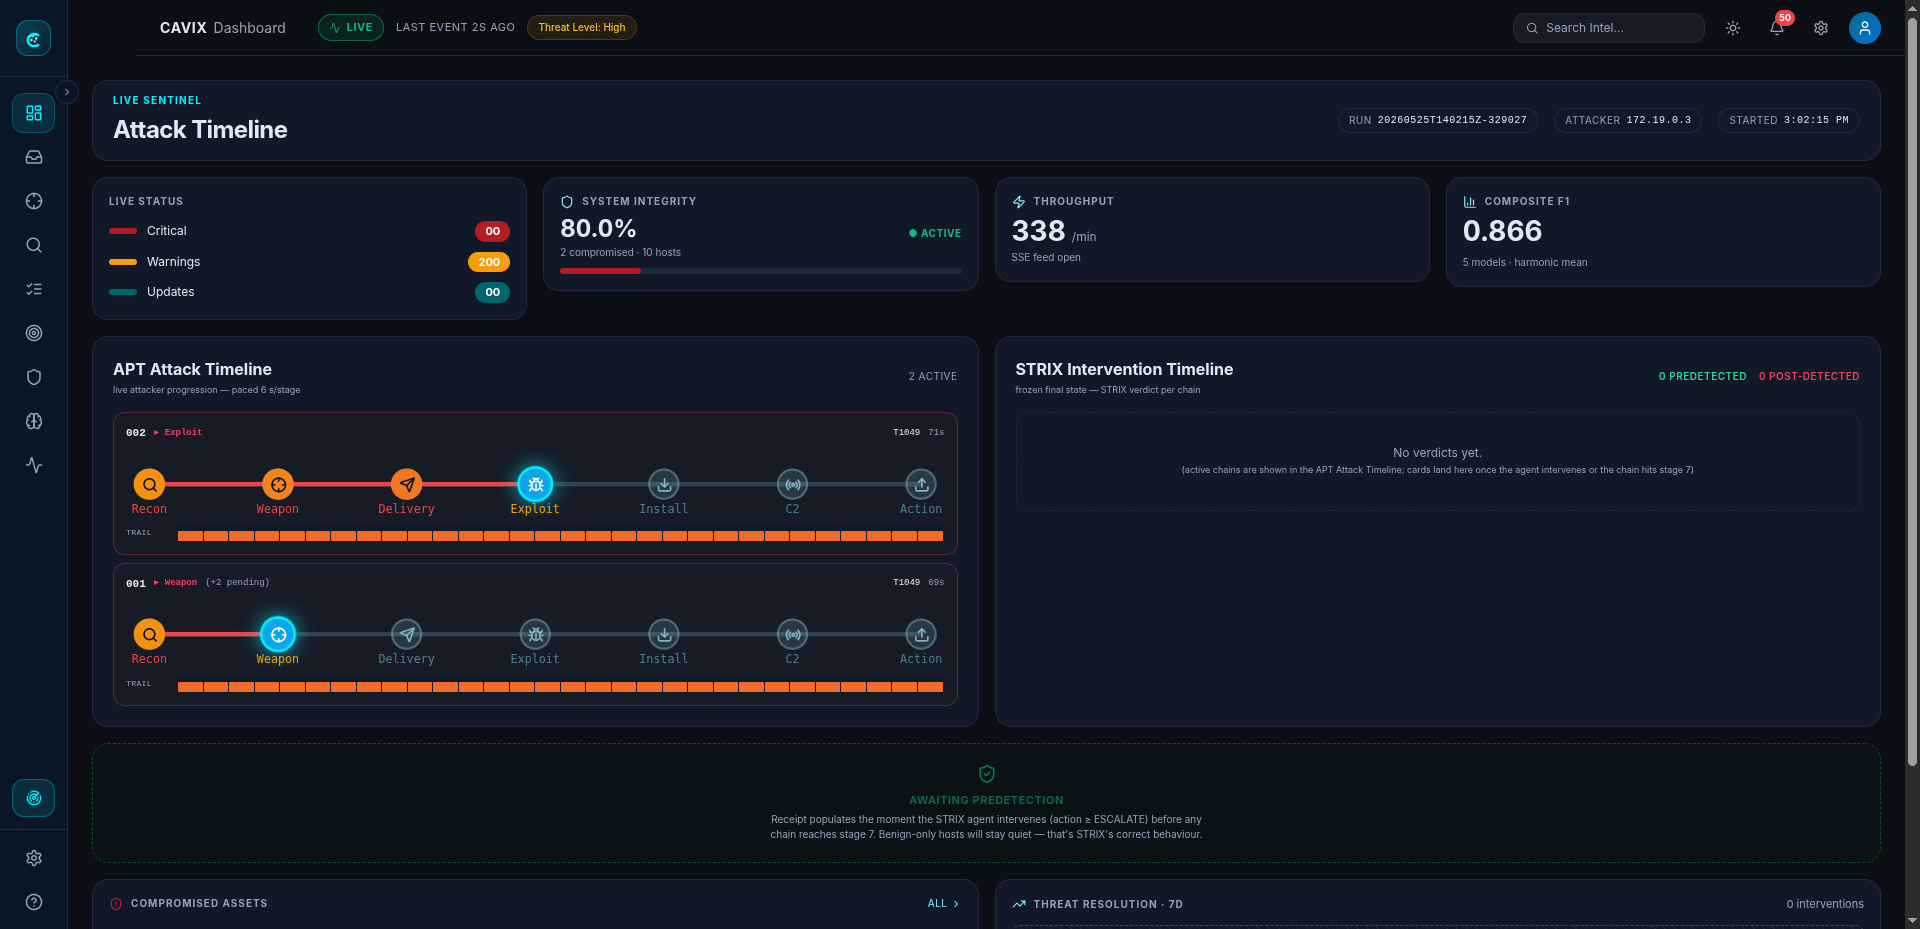
\includegraphics[width=0.95\textwidth]{figures/ch5/simulation-screenshots/1-during-attack}
  \caption{The CAVIX dashboard during an active attack.}
  \label{fig:ch5:sim:attack-during}
  \par\medskip
  As figure~\ref{fig:ch5:sim:attack-during} shows, the two parallel
  attack timelines reconstruct the kill-chain sequence observed on
  each victim, while the right-hand intervention pane remains
  intentionally empty until the gating thresholds are met.
\end{figure}

Figure~\ref{fig:ch5:sim:topology-gnn} provides the spatial view of
the same run. The Simulation Topology on the left reconstructs the
bridge network from the run manifest documented in
chapter~\ref{chap:implementation}: the attacker reaches both
victims through the shared bridge, and the per-tactic chips along
the top reflect the same tactic sequence ordered by occurrence. The
right-hand GNN Victim Graph overlays the GraphSAGE per-host risk
score and reports a maximum risk of 0.77 across the two hosts at
that point in the run, with the attacker node already coloured red
in the live graph.

\begin{figure}[H]
  \centering
  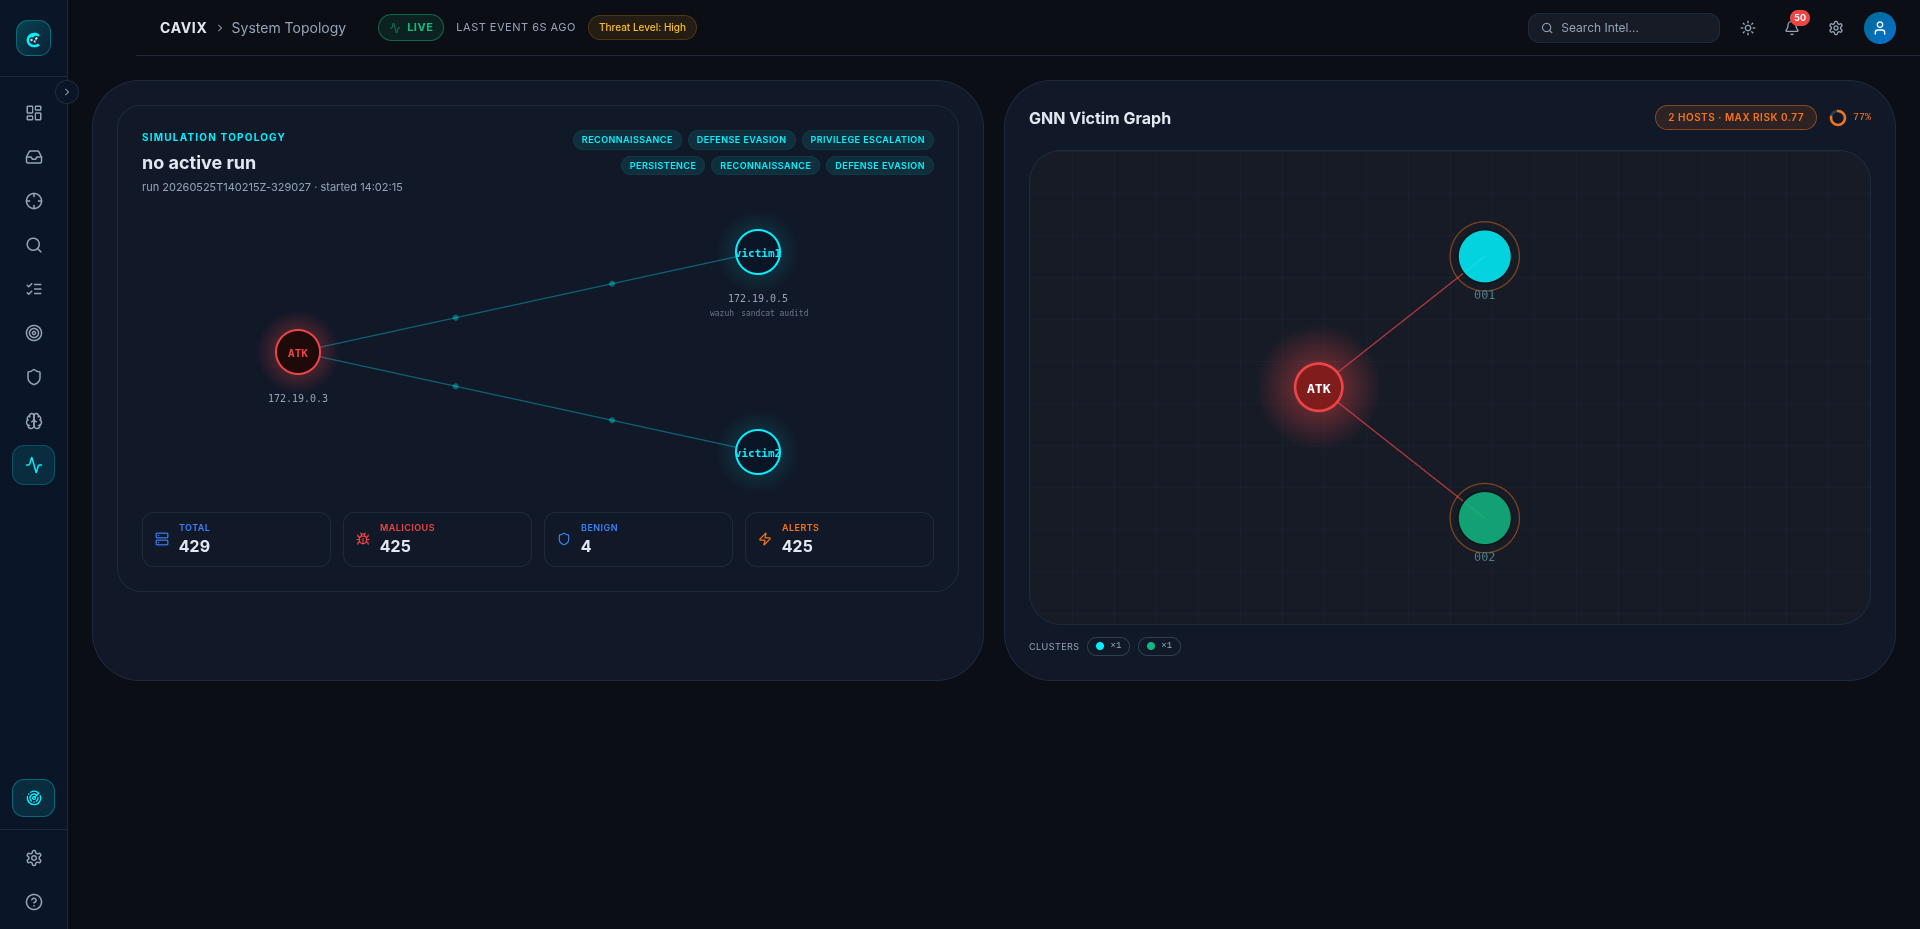
\includegraphics[width=0.95\textwidth]{figures/ch5/simulation-screenshots/2-attack-topology-and-gnn}
  \caption{Simulation topology and GNN victim-graph view of the active run.}
  \label{fig:ch5:sim:topology-gnn}
  \par\medskip
  As shown in figure~\ref{fig:ch5:sim:topology-gnn}, the attacker
  reaches both victims through the bridge; the GraphSAGE graph on the
  right reports a maximum host risk of 0.77 at the moment of capture,
  well above the intervention threshold.
\end{figure}

\subsection{Discussion of Results}
\label{sec:sim:discussion}

Figure~\ref{fig:ch5:sim:models-monitoring} drills into what the
inference workers were emitting at that moment. The four model
panels along the top report the live values that feed the gate: an
autoencoder reconstruction error of 0.07, a $\beta$-VAE malicious
probability of 0.52, a GNN node risk of 0.77, and a Transformer
next-stage confidence of zero. The Transformer value is expected,
because the predicted next stage is one of the absent CKC slots
discussed in chapter~\ref{chap:implementation}, whose loss weight
was set to zero during training. The fifth panel on the right is
the RL Agent indicator, currently sitting at \texttt{LOW\_ALERT}
because the Transformer check has not yet cleared its threshold.
The Inference Stream table below lists the most recent per-event
verdicts as they arrive on the verdict stream.

\begin{figure}[H]
  \centering
  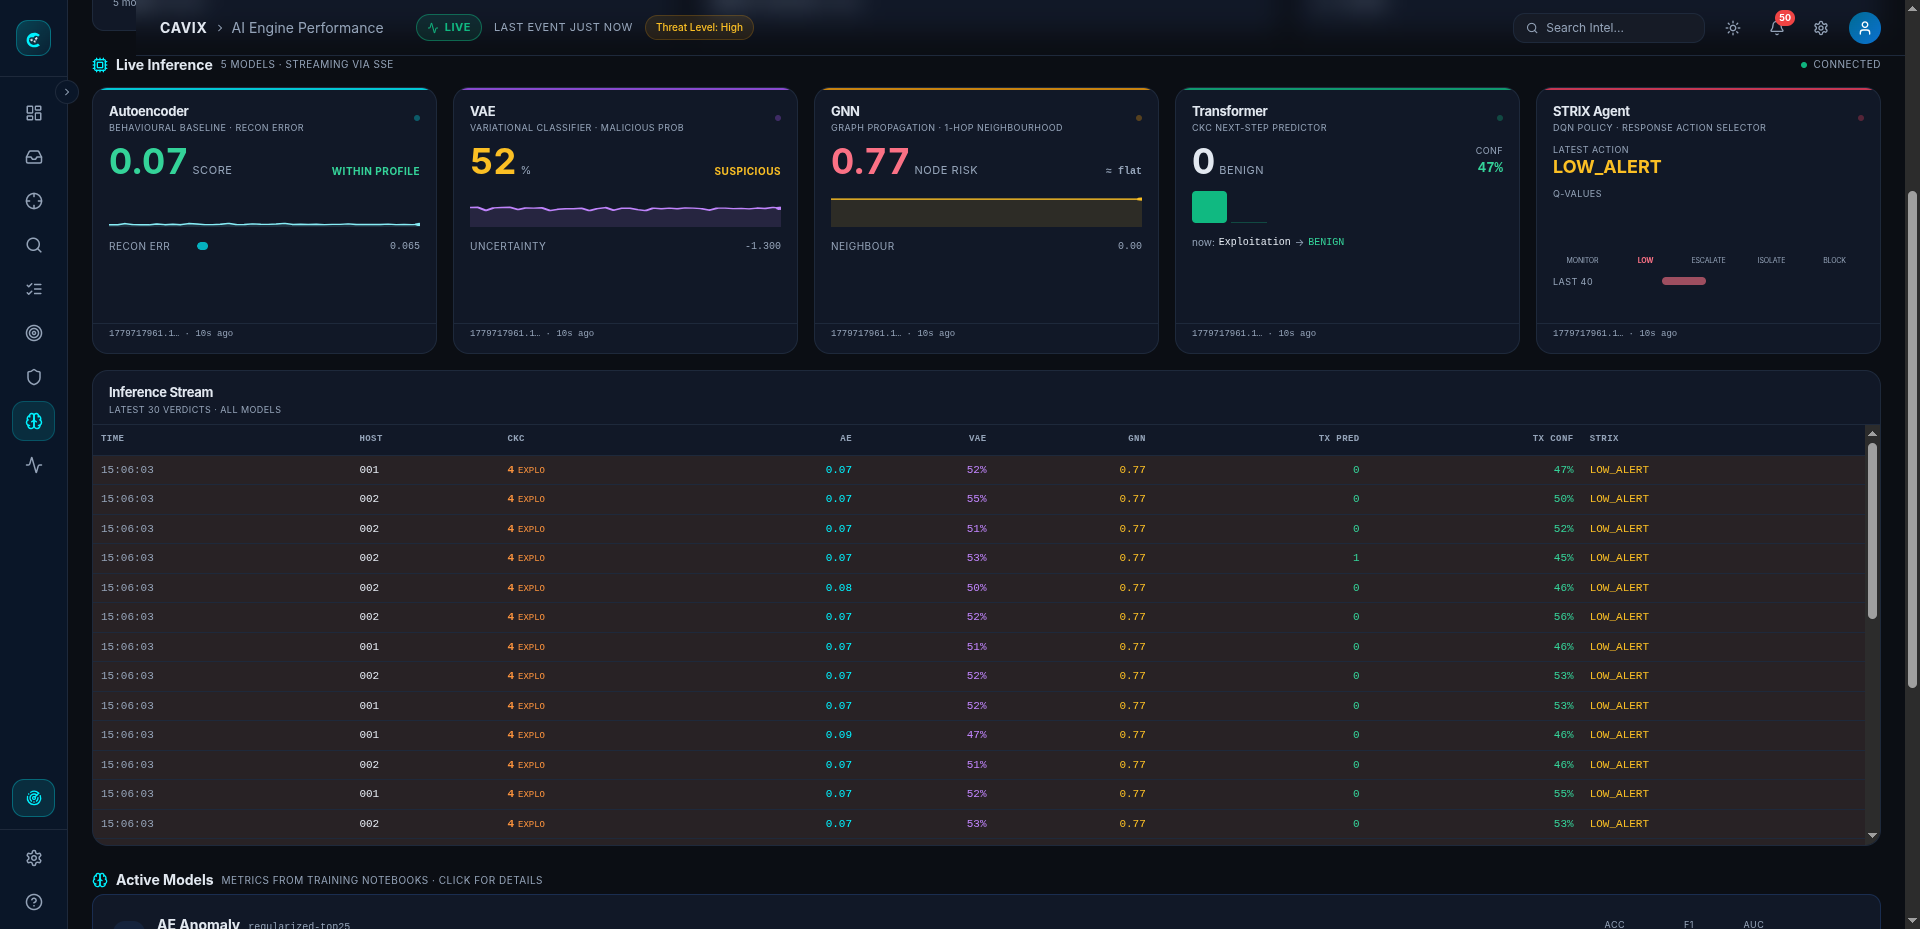
\includegraphics[width=0.95\textwidth]{figures/ch5/simulation-screenshots/4-models-monitoring-results}
  \caption{Model monitoring view of the inference engine during the run.}
  \label{fig:ch5:sim:models-monitoring}
  \par\medskip
  In figure~\ref{fig:ch5:sim:models-monitoring}, the four anomaly-score
  panels report the values consumed by the deterministic gate, and the
  RL Agent panel shows the action that survived gating; the Inference
  Stream below lists the verdicts as they were emitted on the verdict
  stream.
\end{figure}

Figure~\ref{fig:ch5:sim:rl-intervention} closes the loop. Once the
remaining check crossed its threshold, the RL agent's proposed
escalation was authorised and the Intervention Timeline on the
right began populating. The Predetection Receipts pane underneath
records the response history per host, with each receipt mapping a
detected chain to the action that was ultimately issued (an
\texttt{ESCALATE} or an \texttt{ISOLATE\_HOST}, depending on which
gate combination tripped). The Attack Timeline on the left has
cleared to ``no active run'' because the runner has finished its
planned tactic chain.

\begin{figure}[H]
  \centering
  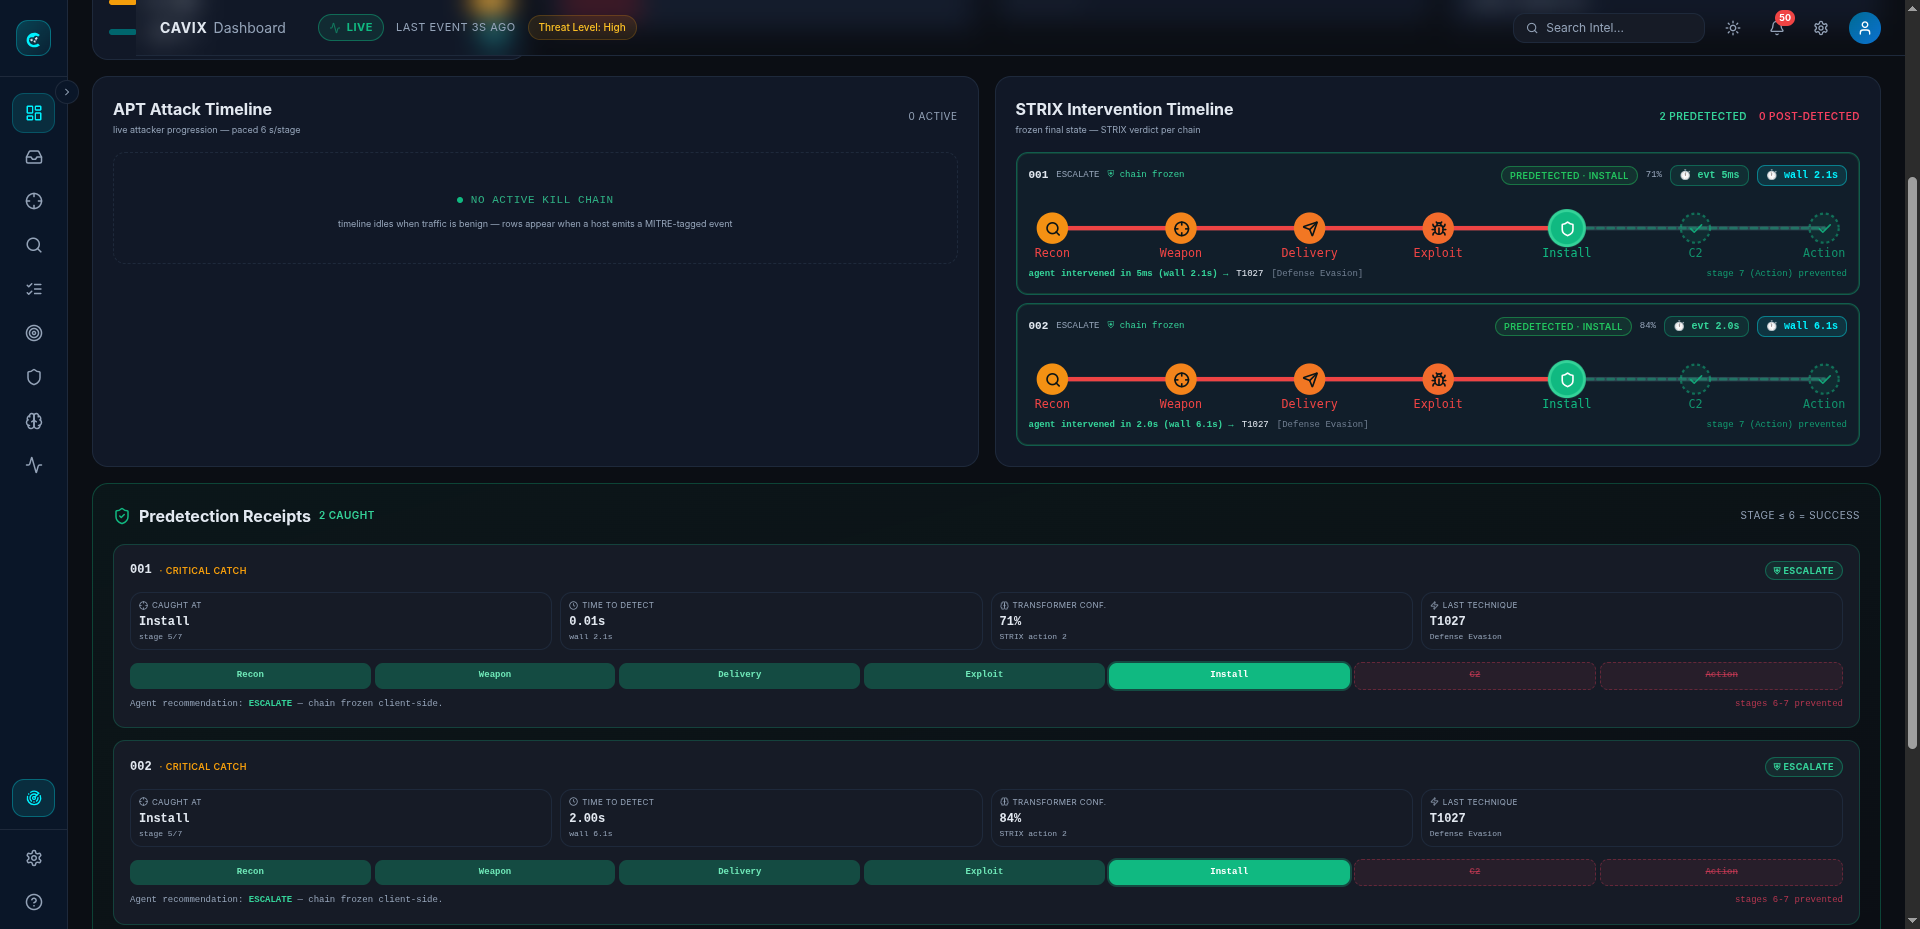
\includegraphics[width=0.95\textwidth]{figures/ch5/simulation-screenshots/3-after-rl-intervention}
  \caption{Dashboard view after the reinforcement-learning agent issued its interventions.}
  \label{fig:ch5:sim:rl-intervention}
  \par\medskip
  As illustrated in figure~\ref{fig:ch5:sim:rl-intervention}, the
  right-hand Intervention Timeline now lists the actions that
  survived gating, and the Predetection Receipts pane records the
  per-host response history with the action that was ultimately
  issued.
\end{figure}

Three observations follow from the run. First, the four detection
models behave consistently with their training profile: the
autoencoder and the GNN drive the gate, the $\beta$-VAE contributes
a calibrated probability in the middle band, and the Transformer
remains silent when the predicted next stage is one of the
kill-chain slots underrepresented in the training set, which is the
behaviour the explicit zero-weighting of those stages was designed
to produce. Second, the deterministic gate behaves as intended: it
suppresses the RL action while only three of the four checks pass,
and authorises it the moment the fourth check crosses its
threshold, which is the only state in which an intervention can
leave the engine. Third, the end-to-end pipeline remained
responsive throughout the run, with no Redis back-pressure visible
on the dashboard and the verdict stream draining within the
five-second writer window introduced in section~\ref{sec:integration}.
The run is therefore consistent with the design assumptions of
chapter~\ref{chap:conception} and exposes no new failure mode beyond
those already documented in section~\ref{sec:rl-agent}.
\section{Conclusion}
